\documentclass[11pt]{article}
%-------------
% SETTINGS
%-------------
	\usepackage{enumitem,amsmath,amsthm,amssymb,amsfonts,hyperref,fancyhdr,graphicx,subfig,footnote,float}
	\usepackage[dvipsnames]{xcolor}
	\usepackage{microtype}
	\usepackage[left=2cm,right=2cm,top=2.5cm,bottom=2cm]{geometry}
	
	\graphicspath{{figures/}}
	\setlength{\parindent}{0cm}
%	\renewcommand*{\thefootnote}{(*)}
	\renewcommand{\baselinestretch}{1.2}
	\renewcommand\textbullet{\ensuremath{\bullet}}
	\setlength{\headheight}{13.6pt}
%-------------
% TIKZ
%-------------
	\usepackage{tikz}
	\usetikzlibrary{arrows,positioning}
	\definecolor{col1}{RGB}{217,255,204} %Green
	\definecolor{col2}{RGB}{204,243,255} %Blue
	\definecolor{col3}{RGB}{250,142,142} %Red
	\definecolor{col4}{RGB}{203,186,255} %Violet
	\definecolor{col5}{RGB}{255,251,189} %Yellow
	\definecolor{col6}{RGB}{219,219,219} %Gray
	%--------------------------------------------------------------------------------------Styles:
	\tikzstyle{conv}=[draw, fill=col1, align=left]
	\tikzstyle{pool}=[draw, fill=col2, align=left]
	\tikzstyle{trans}=[draw, fill=col6, align=center]
	\tikzstyle{fc}=[draw, fill=col5, align=center]
	\tikzstyle{loss}=[draw, fill=col3, align=left]
	\tikzstyle{drop}=[draw, fill=col6, align=left]
	%---------------------------------------------


%-------------
% STYLE
%-------------

	\pagestyle{fancy}
	\lhead{Maha ELBAYAD}
	\rhead{\bf Deep Learning: Homework 2}
	\cfoot{\thepage}



	\title{[M2, MVA]\\ Deep Learning}
	\author{Maha ELBAYAD\\ \href{mailto:maha.elbayad@student.ecp.fr}{\tt maha.elbayad@student.ecp.fr}}
	\date{}

%------------------------
% MATH
% -----------------------
	\newcommand{\p}{\mathbb{P}}
	\newcommand{\e}{\mathbb{E}}
	\newcommand{\R}{\mathbb{R}}
	\newcommand{\X}{\mathcal{X}}
	\newcommand{\Y}{\mathcal{Y}}
	\newcommand{\indep}{\mathrel{\perp\mspace{-10mu}\perp}}
	\newcommand{\nindep}{\centernot{\indep}}


%------------------------
% CONTENT
% -----------------------

\begin{document}
\maketitle
\vspace{-10pt}
\begin{center}
{\huge \bf Homework 3}\\
\today
\vspace{10pt}
\end{center}

\vspace{7pt}

\section{Theory}
	\textbf{Dropout for linear regression:}\\
	Let's prove that the two following optimization problems are equivalent
	\[\underset{w}{\text{minimize }} \e_{R\sim Bernoulli(p)}\left[\|y-(R\odot X)w\|^2\right]\tag{P1}\]
	\[\underset{w}{\text{minimize }} \|y-pXw\|^2+p(1-p)\|\Gamma w\|^2,\:\Gamma=\left[diag(X^TX)\right]^{1/2}\tag{P2}\]
	Where $R\in\{0,1\}^{N\times D}$ encodes the retained variables and $\odot$ denotes the Hadamard product.

	We have:
	\[\begin{split}
	\|y-(R\odot X)w\|^2&=y^Ty-2y^T(R\odot X)w+w^T(R\odot X)^T(R\odot X)w\\
	\e_{R\sim Bernoulli(p)}[...]&=y^Ty-2py^TXw+w^T(var(R\odot X)+p^2X^TX)w\phantom{abcd} \scriptstyle{(\e_R[R\odot X]=pX)}\\
	&=y^Ty-2py^TXw+w^T(p(1-p)diag(X^TX)+p^2X^TX)w\\
	&=(y-pXw)^T(y-pXw)+p(1-p)w^T(diag(X^TX))w\\
	&=\|y-pXw\|^2+p(1-p)\|\Gamma w\|^2\qed
	\end{split}\]
%\newpage
\section{LeNet:}
\subsection{Experimentation \texttt{\footnotesize (MatConvNet v1.0-beta16})}
\textbf{(V1 : baseline)} We train a simplified version of LeCun's LeNet on a subset of the MNIST database.
	We synthetize the network's architecture in the following diagramm: 
	\begin{savenotes}
	\begin{figure}[H]
		\centering
		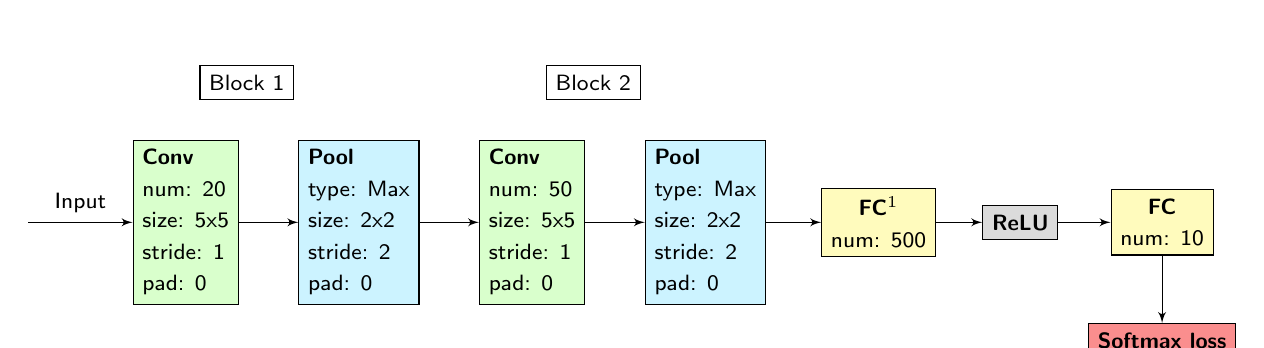
\begin{tikzpicture}[node distance=2.5cm,auto,>=latex',font=\sffamily\footnotesize]
		    \node [conv] (a) {\textbf{Conv}\\num: 20\\size: 5x5\\stride: 1\\pad: 0};
		    \node (start) [left of=a,node distance=2cm, coordinate] {};
		    \node [pool] (b) [right of=a,node distance=2.2cm] {\textbf{Pool}\\type: Max\\size: 2x2\\stride: 2\\pad: 0};
		    \node [conv] (c) [right of=b,node distance=2.2cm]{\textbf{Conv}\\num: 50\\size: 5x5\\stride: 1\\pad: 0};
		    \node [pool] (d) [right of=c,node distance=2.2cm] {\textbf{Pool}\\type: Max\\size: 2x2\\stride: 2\\pad: 0};
		    \node [fc] (e) [right of=d,node distance=2.2cm]{\textbf{FC}\footnotemark\\num: 500};
		    \node [trans] (f) [right of=e,node distance=1.8cm]{\textbf{ReLU}};
		    \node [fc] (g) [right of=f,node distance=1.8cm]{\textbf{FC}\\num: 10};
		    \node [loss] (h) [below of=g,node distance=1.5cm]{\textbf{Softmax loss}};
		    \node[draw] [above right =.5cm and -0.5cm of a] {Block 1};
		    \node[draw] [above right =.5cm and -0.5cm of c] {Block 2};
		    \path[->] 
		    (start) edge node {Input} (a)
		    (a) edge node {} (b)
		    (b) edge node {} (c)
		    (c) edge node {} (d)
		    (d) edge node {} (e)
		    (e) edge node {} (f)
		    (f) edge node {} (g)
		    (g) edge node {} (h);
		\end{tikzpicture}
	\end{figure}
	\end{savenotes}
	\footnotetext{FC for the fully connected layers}
	We train the network in 100 epoches and get the results shown in figure (\ref{v1})
	\begin{figure}[H]
	    \centering
	    \includegraphics[width=15cm]{v1}
	    \caption{Baseline (2-Blocks) network\label{v1}}
	\end{figure}

%=============================
\textbf{(V2)} Reduce the depth of the net : A single block \{\texttt{conv,pool}\} - modified the pool layer to reduce the number of the network'parameters:
	\begin{figure}[H]
		\centering
		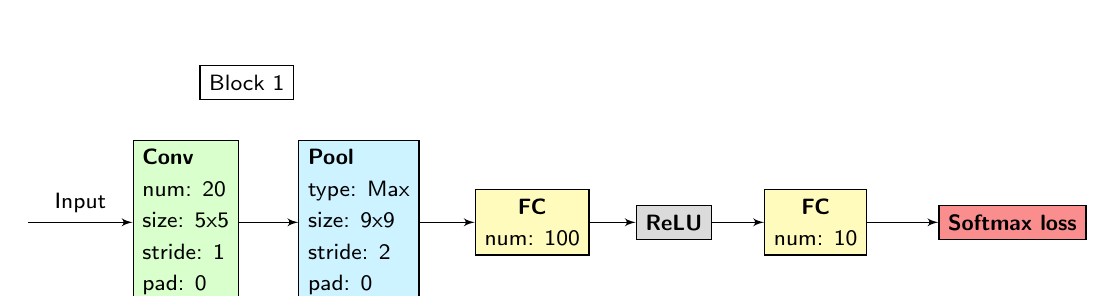
\begin{tikzpicture}[node distance=2.5cm,auto,>=latex',font=\sffamily\footnotesize]
		    \node [conv] (a) {\textbf{Conv}\\num: 20\\size: 5x5\\stride: 1\\pad: 0};
		    \node (start) [left of=a,node distance=2cm, coordinate] {};
		    \node [pool] (b) [right of=a,node distance=2.2cm] {\textbf{Pool}\\type: Max\\size: 9x9\\stride: 2\\pad: 0};
		    \node [fc] (e) [right of=b,node distance=2.2cm]{\textbf{FC}\\num: 100};
		    \node [trans] (f) [right of=e,node distance=1.8cm]{\textbf{ReLU}};
		    \node [fc] (g) [right of=f,node distance=1.8cm]{\textbf{FC}\\num: 10};
		    \node [loss] (h) [right of=g,node distance=2.5cm]{\textbf{Softmax loss}};
		    \node[draw] [above right =.5cm and -0.5cm of a] {Block 1};
		    \path[->] 
		    (start) edge node {Input} (a)
		    (a) edge node {} (b)
		    (b) edge node {} (e)
		    (e) edge node {} (f)
		    (f) edge node {} (g)
		    (g) edge node {} (h);
		\end{tikzpicture}
	\end{figure}
	\begin{figure}[H]
	    \centering
	    \includegraphics[width=15cm]{v2}
	    \caption{1-Block network}
	\end{figure}

%=============================
\textbf{(V3)} Add an extra block \{\texttt{conv,pool}\}:
	\begin{figure}[H]
	    \centering
	    \includegraphics[width=15cm]{v3}
	    \caption{3-Blocks network}
	\end{figure}
	\begin{figure}[H]
		\centering
		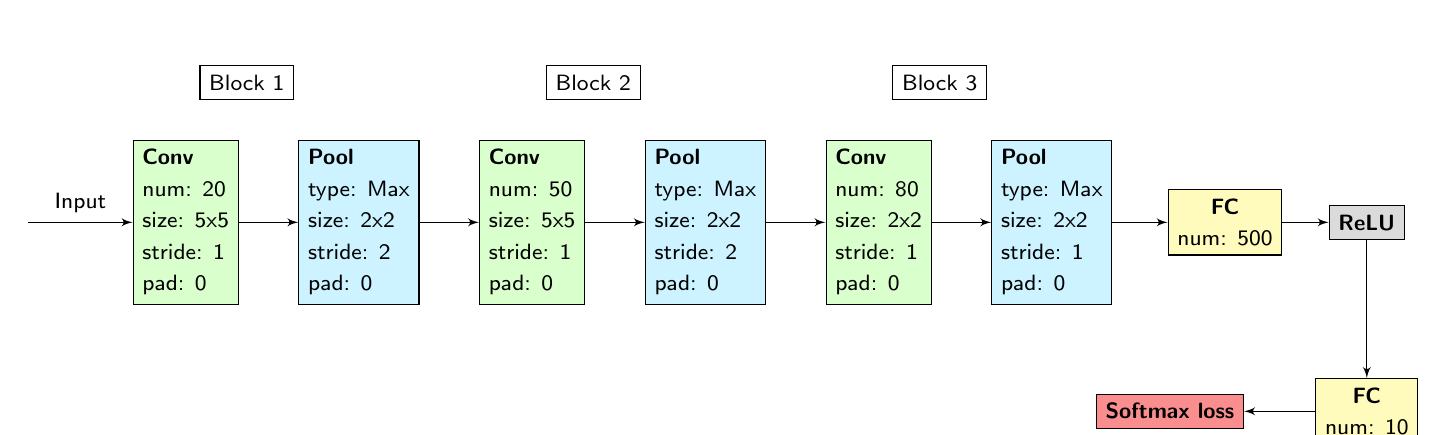
\begin{tikzpicture}[node distance=2.5cm,auto,>=latex',font=\sffamily\footnotesize]
		    \node [conv] (a) {\textbf{Conv}\\num: 20\\size: 5x5\\stride: 1\\pad: 0};
		    \node (start) [left of=a,node distance=2cm, coordinate] {};
		    \node [pool] (b) [right of=a,node distance=2.2cm] {\textbf{Pool}\\type: Max\\size: 2x2\\stride: 2\\pad: 0};
		    \node [conv] (c) [right of=b,node distance=2.2cm]{\textbf{Conv}\\num: 50\\size: 5x5\\stride: 1\\pad: 0};
		    \node [pool] (d) [right of=c,node distance=2.2cm] {\textbf{Pool}\\type: Max\\size: 2x2\\stride: 2\\pad: 0};
		    \node [conv] (ce) [right of=d,node distance=2.2cm]{\textbf{Conv}\\num: 80\\size: 2x2\\stride: 1\\pad: 0};
		    \node [pool] (de) [right of=ce,node distance=2.2cm] {\textbf{Pool}\\type: Max\\size: 2x2\\stride: 1\\pad: 0};
		    \node [fc] (e) [right of=de,node distance=2.2cm]{\textbf{FC}\\num: 500};
		    \node [trans] (f) [right of=e,node distance=1.8cm]{\textbf{ReLU}};
		    \node [fc] (g) [below of=f,node distance=2.4cm]{\textbf{FC}\\num: 10};
		    \node [loss] (h) [left of=g,node distance=2.5cm]{\textbf{Softmax loss}};
		    \node[draw] [above right =.5cm and -0.5cm of a] {Block 1};
		    \node[draw] [above right =.5cm and -0.5cm of c] {Block 2};
		    \node[draw] [above right =.5cm and -0.5cm of ce] {Block 3};
		    \path[->] 
		    (start) edge node {Input} (a)
		    (a) edge node {} (b)
		    (b) edge node {} (c)
		    (c) edge node {} (d)
		    (d) edge node {} (ce)
		    (ce) edge node {} (de)
		    (de) edge node {} (e)
		    (e) edge node {} (f)
		    (f) edge node {} (g)
		    (g) edge node {} (h);
		\end{tikzpicture}
	\end{figure}

%=============================

\textbf{(V4)} 2 Blocks \{\texttt{conv,pool,relu}\}:
	\begin{figure}[H]
		\centering
		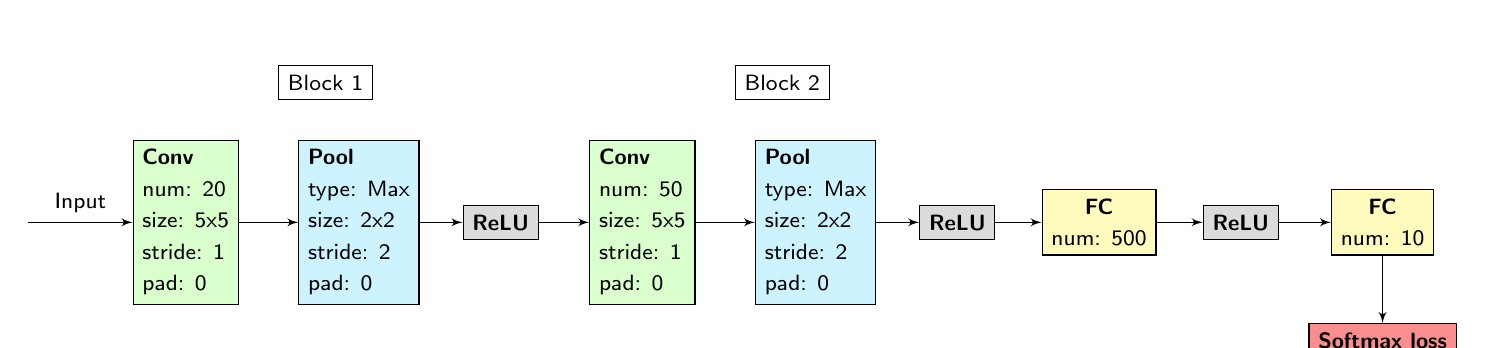
\begin{tikzpicture}[node distance=2.5cm,auto,>=latex',font=\sffamily\footnotesize]
		    \node [conv] (a) {\textbf{Conv}\\num: 20\\size: 5x5\\stride: 1\\pad: 0};
		    \node (start) [left of=a,node distance=2cm, coordinate] {};
		    \node [pool] (b) [right of=a,node distance=2.2cm] {\textbf{Pool}\\type: Max\\size: 2x2\\stride: 2\\pad: 0};
		    \node [trans] (be) [right of=b,node distance=1.8cm]{\textbf{ReLU}};
		    \node [conv] (c) [right of=be,node distance=1.8cm]{\textbf{Conv}\\num: 50\\size: 5x5\\stride: 1\\pad: 0};
		    \node [pool] (d) [right of=c,node distance=2.2cm] {\textbf{Pool}\\type: Max\\size: 2x2\\stride: 2\\pad: 0};
		    \node [trans] (de) [right of=d,node distance=1.8cm]{\textbf{ReLU}};
		    \node [fc] (e) [right of=de,node distance=1.8cm]{\textbf{FC}\\num: 500};
		    \node [trans] (f) [right of=e,node distance=1.8cm]{\textbf{ReLU}};
		    \node [fc] (g) [right of=f,node distance=1.8cm]{\textbf{FC}\\num: 10};
		    \node [loss] (h) [below of=g,node distance=1.5cm]{\textbf{Softmax loss}};
		    \node[draw] [above right =.5cm and 0.5cm of a] {Block 1};
		    \node[draw] [above right =.5cm and 0.5cm of c] {Block 2};
		    \path[->] 
		    (start) edge node {Input} (a)
		    (a) edge node {} (b)
		    (b) edge node {} (be)
		    (be) edge node {} (c)
		    (c) edge node {} (d)
		    (d) edge node {} (de)
		    (de) edge node {} (e)
		    (e) edge node {} (f)
		    (f) edge node {} (g)
		    (g) edge node {} (h);
		\end{tikzpicture}
	\end{figure}

	\begin{figure}[H]
	    \centering
	    \includegraphics[width=15cm]{v4}
	    \caption{2-Blocks network - \{conv,pool relu\}}
	\end{figure}

%=============================
\newpage
\textbf{(V5)} Baseline with dropout (rate=.5) after the ReLU.
	\begin{figure}[H]
	    \centering
	    \includegraphics[width=15cm]{v5}
	    \caption{Baseline network - Added dropout}
	\end{figure}

%=============================
\textbf{Maxout pooling implementation:}\\
The output of the layer preceding the maxout is:
\[z=x^T\mathbf W+b\in\R^{H\times W\times K\times N}\]
Where:\\
- $(H\times W)$ size of the feature map.\\
- $K$: number of channels.\\
- $N$ the batch size.\\
- $\mathbf W, b$ weights and biases of the preceding layer. 
\begin{description}
\item[Forward - Channels pooling $(|groups|=G)$] \[y_i=\max_{j\in K_i}z_{..j.},\:i\in{1,..G},\:K_i\text{ indices of the $i^{th}$ group },y\in \R^{H\times W\times G\times N}\]
\texttt{Auxiliary output Mask:} boolean indicator of the filtered values $(\texttt{Mask}\in \R^{H\times W\times K\times N})$
\item[Backward] Given $\frac{dz}{dy}\in \R^{H\times W\times G\times N}$, 
\[\frac{dz}{dx}=\underset{K_1,...K_G}{\text{Duplicate along the channels dimension }} \frac{dz}{dy}\odot \texttt{Mask}\in\R^{H\times W\times K\times N}\]
\end{description}
\newpage

%=============================

\textbf{(V6, 6bis)} After implementing the maxout layer, we add it to th network after the 2nd block.
	\begin{figure}[H]
		\centering
		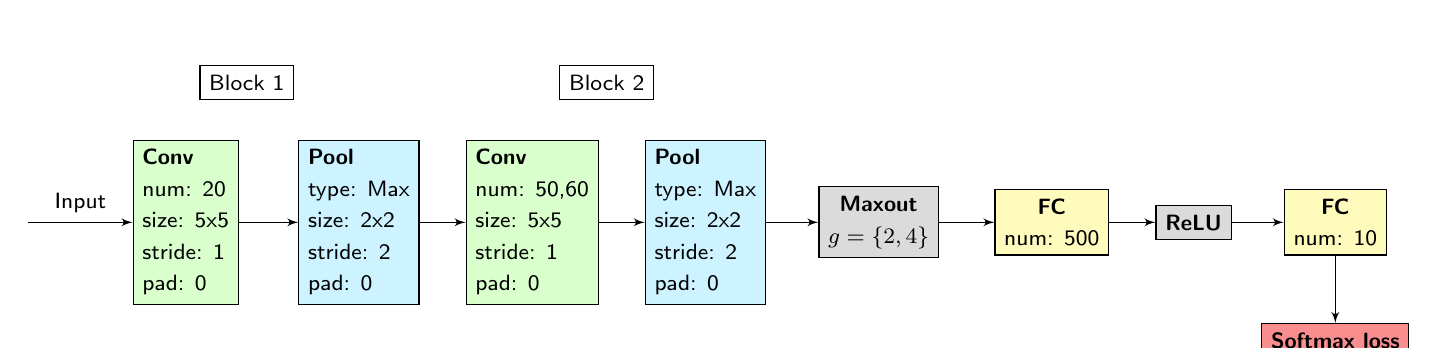
\begin{tikzpicture}[node distance=2.5cm,auto,>=latex',font=\sffamily\footnotesize]
		    \node [conv] (a) {\textbf{Conv}\\num: 20\\size: 5x5\\stride: 1\\pad: 0};
		    \node (start) [left of=a,node distance=2cm, coordinate] {};
		    \node [pool] (b) [right of=a,node distance=2.2cm] {\textbf{Pool}\\type: Max\\size: 2x2\\stride: 2\\pad: 0};
		    \node [conv] (c) [right of=b,node distance=2.2cm]{\textbf{Conv}\\num: 50,60\\size: 5x5\\stride: 1\\pad: 0};
		    \node [pool] (d) [right of=c,node distance=2.2cm] {\textbf{Pool}\\type: Max\\size: 2x2\\stride: 2\\pad: 0};
		    \node [trans] (dd) [right of=d,node distance=2.2cm]{\textbf{Maxout}\\$g=\{2,4\}$};
		    \node [fc] (e) [right of=dd,node distance=2.2cm]{\textbf{FC}\\num: 500};
		    \node [trans] (f) [right of=e,node distance=1.8cm]{\textbf{ReLU}};
		    \node [fc] (g) [right of=f,node distance=1.8cm]{\textbf{FC}\\num: 10};
		    \node [loss] (h) [below of=g,node distance=1.5cm]{\textbf{Softmax loss}};
		    \node[draw] [above right =.5cm and -0.5cm of a] {Block 1};
		    \node[draw] [above right =.5cm and -0.5cm of c] {Block 2};
		    \path[->] 
		    (start) edge node {Input} (a)
		    (a) edge node {} (b)
		    (b) edge node {} (c)
		    (c) edge node {} (d)
		    (d) edge node {} (dd)
		    (dd) edge node {} (e)
		    (e) edge node {} (f)
		    (f) edge node {} (g)
		    (g) edge node {} (h);
		\end{tikzpicture}
	\end{figure}

	\begin{figure}[H]
	    \centering
	    \subfloat[g=2]{
	    \includegraphics[width=14cm]{v6}}
	    \\
	    \subfloat[g=4]{
	    \includegraphics[width=14cm]{v6bis}}
	\caption{Baseline network - Maxout @Block2}
	\end{figure}

%=============================

\textbf{(V7)} Now we add a maxout layer to th network after the 1st block (baseline model)
	\begin{figure}[H]
		\centering
		\begin{tikzpicture}[node distance=2.5cm,auto,>=latex',font=\sffamily\footnotesize]
		    \node [conv] (a) {\textbf{Conv}\\num: 20\\size: 5x5\\stride: 1\\pad: 0};
		    \node (start) [left of=a,node distance=2cm, coordinate] {};
		    \node [pool] (b) [right of=a,node distance=2.2cm] {\textbf{Pool}\\type: Max\\size: 2x2\\stride: 2\\pad: 0};
		    \node [trans] (bb) [right of=b,node distance=2.2cm]{\textbf{Maxout}\\g=2};
		    \node [conv] (c) [right of=bb,node distance=2.2cm]{\textbf{Conv}\\num: 50\\size: 5x5\\stride: 1\\pad: 0};
		    \node [pool] (d) [right of=c,node distance=2.2cm] {\textbf{Pool}\\type: Max\\size: 2x2\\stride: 2\\pad: 0};
		    \node [fc] (e) [right of=d,node distance=2.2cm]{\textbf{FC}\\num: 500};
		    \node [trans] (f) [right of=e,node distance=1.8cm]{\textbf{ReLU}};
		    \node [fc] (g) [right of=f,node distance=1.8cm]{\textbf{FC}\\num: 10};
		    \node [loss] (h) [below of=g,node distance=1.5cm]{\textbf{Softmax loss}};
		    \node[draw] [above right =.5cm and -0.5cm of a] {Block 1};
		    \node[draw] [above right =.5cm and -0.5cm of c] {Block 2};
		    \path[->] 
		    (start) edge node {Input} (a)
		    (a) edge node {} (b)
		    (b) edge node {} (bb)
		    (bb) edge node {} (c)
		    (c) edge node {} (d)
		    (d) edge node {} (dd)
		    (dd) edge node {} (e)
		    (e) edge node {} (f)
		    (f) edge node {} (g)
		    (g) edge node {} (h);
		\end{tikzpicture}
	\end{figure}
	\begin{figure}[H]
	    \centering
	    \includegraphics[width=15cm]{v7}
	    \caption{Baseline network - Maxout @Block1}
	\end{figure}

%=============================

\textbf{(V8)} We combine both the maxout after the 2nd block and the dropout after the ReLU.
	
	\begin{figure}[H]
		\centering
		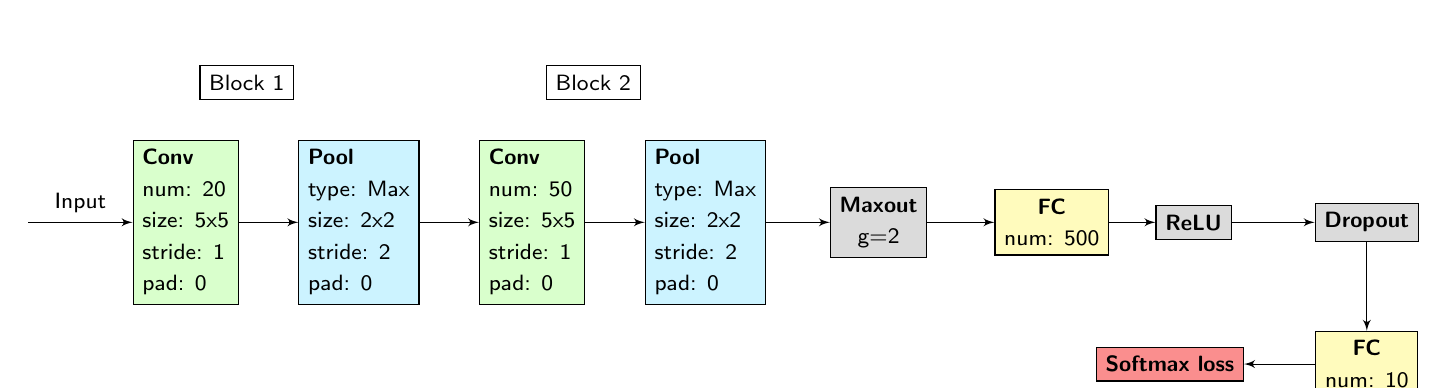
\begin{tikzpicture}[node distance=2.5cm,auto,>=latex',font=\sffamily\footnotesize]
		    \node [conv] (a) {\textbf{Conv}\\num: 20\\size: 5x5\\stride: 1\\pad: 0};
		    \node (start) [left of=a,node distance=2cm, coordinate] {};
		    \node [pool] (b) [right of=a,node distance=2.2cm] {\textbf{Pool}\\type: Max\\size: 2x2\\stride: 2\\pad: 0};
		    \node [conv] (c) [right of=b,node distance=2.2cm]{\textbf{Conv}\\num: 50\\size: 5x5\\stride: 1\\pad: 0};
		    \node [pool] (d) [right of=c,node distance=2.2cm] {\textbf{Pool}\\type: Max\\size: 2x2\\stride: 2\\pad: 0};
		    \node [trans] (dd) [right of=d,node distance=2.2cm]{\textbf{Maxout}\\g=2};
		    \node [fc] (e) [right of=dd,node distance=2.2cm]{\textbf{FC}\\num: 500};
		    \node [trans] (f) [right of=e,node distance=1.8cm]{\textbf{ReLU}};
		    \node [trans] (ff) [right of=f,node distance=2.2cm]{\textbf{Dropout}};
		    \node [fc] (g) [below of=ff,node distance=1.8cm]{\textbf{FC}\\num: 10};
		    \node [loss] (h) [left of=g,node distance=2.5cm]{\textbf{Softmax loss}};
		    \node[draw] [above right =.5cm and -0.5cm of a] {Block 1};
		    \node[draw] [above right =.5cm and -0.5cm of c] {Block 2};
		    \path[->] 
		    (start) edge node {Input} (a)
		    (a) edge node {} (b)
		    (b) edge node {} (c)
		    (c) edge node {} (d)
		    (d) edge node {} (dd)
		    (dd) edge node {} (e)
		    (e) edge node {} (f)
		    (f) edge node {} (ff)
		    (ff) edge node {} (g)
		    (g) edge node {} (h);
		\end{tikzpicture}
	\end{figure}
	\begin{figure}[H]
	    \centering
	    \includegraphics[width=15cm]{v8}
	    \caption{Baseline network - Maxout @Block1 + Dropout}
	\end{figure}

%=============================

\textbf{(V9)} We combine dropout with blocks \texttt{(Conv,Pool,Maxout)}
	\begin{figure}[H]
	    \centering
	    \includegraphics[width=15cm]{v9}
	    \caption{Baseline network - Maxout @Block1,2 + Dropout}
	\end{figure}
	\begin{figure}[H]
		\centering
		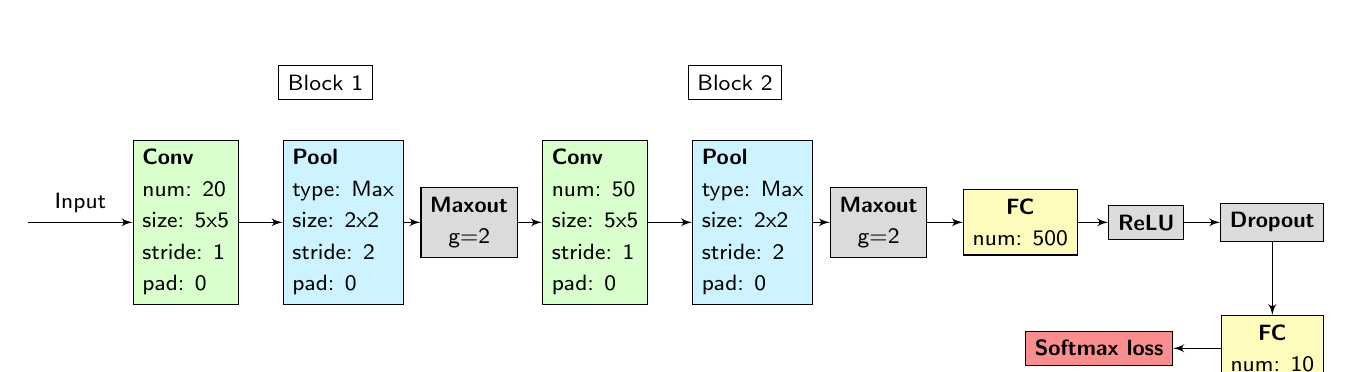
\begin{tikzpicture}[node distance=2.5cm,auto,>=latex',font=\sffamily\footnotesize]
		    \node [conv] (a) {\textbf{Conv}\\num: 20\\size: 5x5\\stride: 1\\pad: 0};
		    \node (start) [left of=a,node distance=2cm, coordinate] {};
		    \node [pool] (b) [right of=a,node distance=2cm] {\textbf{Pool}\\type: Max\\size: 2x2\\stride: 2\\pad: 0};
		    \node [trans] (be) [right of=b,node distance=1.6cm]{\textbf{Maxout}\\g=2};
		    \node [conv] (c) [right of=be,node distance=1.6cm]{\textbf{Conv}\\num: 50\\size: 5x5\\stride: 1\\pad: 0};
		    \node [pool] (d) [right of=c,node distance=2cm] {\textbf{Pool}\\type: Max\\size: 2x2\\stride: 2\\pad: 0};
		    \node [trans] (dd) [right of=d,node distance=1.6cm]{\textbf{Maxout}\\g=2};
		    \node [fc] (e) [right of=dd,node distance=1.8cm]{\textbf{FC}\\num: 500};
		    \node [trans] (f) [right of=e,node distance=1.6cm]{\textbf{ReLU}};
		    \node [trans] (ff) [right of=f,node distance=1.6cm]{\textbf{Dropout}};
		    \node [fc] (g) [below of=ff,node distance=1.6cm]{\textbf{FC}\\num: 10};
		    \node [loss] (h) [left of=g,node distance=2.2cm]{\textbf{Softmax loss}};
		    \node[draw] [above right =.5cm and 0.5cm of a] {Block 1};
		    \node[draw] [above right =.5cm and 0.5cm of c] {Block 2};
		    \path[->] 
		    (start) edge node {Input} (a)
		    (a) edge node {} (b)
		    (b) edge node {} (be)
		    (be) edge node {} (c)
		    (c) edge node {} (d)
		    (d) edge node {} (dd)
		    (dd) edge node {} (e)
		    (e) edge node {} (f)
		    (f) edge node {} (ff)
		    (ff) edge node {} (g)
		    (g) edge node {} (h);
		\end{tikzpicture}
	\end{figure}
%=============================

\textbf{(V10)} $\sim$ (V9) with ReLU instead of Maxout.
	\begin{figure}[H]
	    \centering
	    \includegraphics[width=15cm]{v10}
	    \caption{$2\times(\texttt{Conv, Pool, ReLU})$+ Dropout}
	\end{figure}

%=============================

\textbf{(V11)} The model of (Goodfellow et al, 2013)
	\begin{figure}[H]
		\centering
		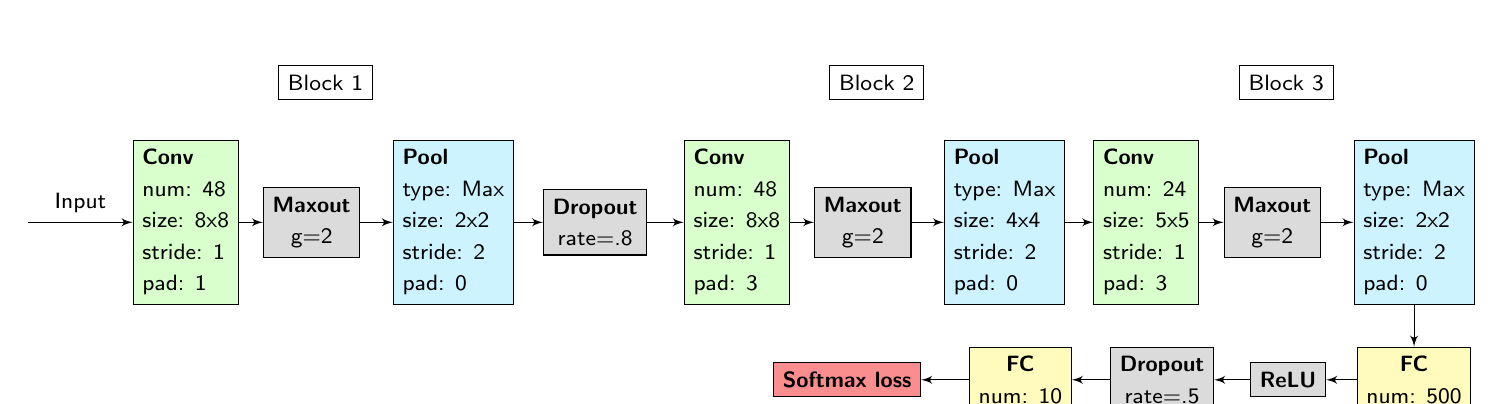
\begin{tikzpicture}[node distance=2.5cm,auto,>=latex',font=\sffamily\footnotesize]
		    \node [conv] (a) {\textbf{Conv}\\num: 48\\size: 8x8\\stride: 1\\pad: 1};
		    \node (start) [left of=a,node distance=2cm, coordinate] {};
		    \node [trans] (b) [right of=a,node distance=1.6cm]{\textbf{Maxout}\\g=2};
		    \node [pool] (be) [right of=b,node distance=1.8cm] {\textbf{Pool}\\type: Max\\size: 2x2\\stride: 2\\pad: 0};
		    \node [trans] (bb) [right of=be,node distance=1.8cm]{\textbf{Dropout}\\rate=.8};
		    \node [conv] (c) [right of=bb,node distance=1.8cm]{\textbf{Conv}\\num: 48\\size: 8x8\\stride: 1\\pad: 3}; 
		    \node [trans] (d) [right of=c,node distance=1.6cm]{\textbf{Maxout}\\g=2};
		    \node [pool] (dd) [right of=d,node distance=1.8cm] {\textbf{Pool}\\type: Max\\size: 4x4\\stride: 2\\pad: 0};
		    \node [conv] (c2) [right of=dd,node distance=1.8cm]{\textbf{Conv}\\num: 24\\size: 5x5\\stride: 1\\pad: 3}; 
		    \node [trans] (d2) [right of=c2,node distance=1.6cm]{\textbf{Maxout}\\g=2};
		    \node [pool] (dd2) [right of=d2,node distance=1.8cm] {\textbf{Pool}\\type: Max\\size: 2x2\\stride: 2\\pad: 0};
		    \node [fc] (e) [below of=dd2,node distance=2cm]{\textbf{FC}\\num: 500};
		    \node [trans] (f) [left of=e,node distance=1.6cm]{\textbf{ReLU}};
		    \node [trans] (ff) [left of=f,node distance=1.6cm]{\textbf{Dropout}\\rate=.5};
		    \node [fc] (g) [left of=ff,node distance=1.8cm]{\textbf{FC}\\num: 10};
		    \node [loss] (h) [left of=g,node distance=2.2cm]{\textbf{Softmax loss}};
		    \node[draw] [above right =.5cm and 0.5cm of a] {Block 1};
		    \node[draw] [above right =.5cm and 0.5cm of c] {Block 2};
		    \node[draw] [above right =.5cm and 0.5cm of c2] {Block 3};
		    \path[->] 
		    (start) edge node {Input} (a)
		    (a) edge node {} (b)
		    (b) edge node {} (be)
		    (be) edge node {} (bb)
		    (bb) edge node {} (c)
		    (c) edge node {} (d)
		    (d) edge node {} (dd)
		    (dd) edge node {} (c2)
		    (c2) edge node {} (d2)
		    (d2) edge node {} (dd2)
		    (dd2) edge node {} (e)
		    (e) edge node {} (f)
		    (f) edge node {} (ff)
		    (ff) edge node {} (g)
		    (g) edge node {} (h);
		\end{tikzpicture}
	\end{figure}
	\begin{figure}[H]
	    \centering
	    \includegraphics[width=15cm]{v11}
	    \caption{Goodfellow 2013}
	\end{figure}
%==================================== RECAP

\subsection{Summary:}
	\begin{savenotes}
	\begin{table}[H]
	\centering
	\begin{tabular}{|l|c|c||c|}
		\hline
		Model & Validation Error & E(val)  & E(train)\footnotemark\\ 
		\hline
		v1 : $2\times(\texttt{Conv, Pool})$ & 1.99\% & 8.86e-02 & 1.31e-04 \\
		v2 : $1\times(\texttt{Conv, Pool})$ & 2.18\% & 1.38e-01 & 1.51e-02 \\
		v3 : $3\times(\texttt{Conv, Pool})$ & 2.57\% & 1.30e-01 & 2.09e-04 \\
		v4 : $2\times(\texttt{Conv, Pool, ReLU})$ & 1.87\% & 7.90e-02 & 1.54e-04\\
		v5 : v1 + dropout  & 1.40\% & 6.62e-02 & 6.67e-04 \\
		v6 : v1 + maxout @block2 (g=2)& 1.63\% & 7.74e-02 & 1.35e-04 \\
		v6 bis : v1 + maxout @block2 (g=4) & 2.00\% & 9.23e-02 & 1.35e-04 \\
		v7 : v1 + maxout @block1 & 1.65\% & 6.63e-02 & 1.56e-04\\
		v8 : v6 + dropout & 1.26\% & 5.46e-02 & 1.21e-03 \\
		v9 : $2\times(\texttt{Conv, Pool, Max})$ + dropout & 1.29\% & 6.71e-02 & 8.67e-04 \\
		v10 : $2\times(\texttt{Conv, Pool, ReLU})$ + dropout & \textcolor{BrickRed}{\bf1.05\%} & 4.34e-02 & 8.16e-04\\
		v11 : Goodfellow & \textcolor{BrickRed}{\bf1.02\%} & 4.35e-02 & 9.41e-03\\ 
		\hline
	\end{tabular}
	\end{table}
	\end{savenotes}
	\footnotetext{Objective function at epoch 100}
	\begin{figure}[H]
	    \centering
	    \includegraphics[width=12cm]{recap}
	    \caption{}
	\end{figure}
	\begin{enumerate}[label={\textbullet}]
	\item (v1,v2,v3): The optimal depth of the LeNet network on the MNIST subset is of 2 blocks (performance degrading with depth$>$2).
	\item (v4): Adding ReLUs after pooling layers sparsifies the model and improves the results significantly.
	\item (v5) Adding dropout sparsifies the network responses and boosts its performance. And with its regularization effect, we avoid overfitting the training set.
	\item (v6, v6bis, v7): adding a maxout layer generally improves the results. With g=2 the model's complexity is higher, and so is its performance.
	\item (v8,v9): combining maxout and dropout (@ the $1^{st}$ FC) ensures the sparsity of the responses without dead units at the convolutional part of the network (Although the final test error is in favor of v8, the evolution throughout the training shows that the two models are quite equivalent).
	\item (v10): The model with ReLUs outperforms the maxout network.
	\item (v11): We use larger convolution filters with an extra block and a different arrangement of layers, consequently the performance of the maxout network is enhanced. (although the filters are large, the extra dropout sparsifies the model)
	\end{enumerate}
\end{document}

\textcolor{BrickRed}{\bf }